	\begin{Huge}
			Informatik (Bachelor of Education)
		\end{Huge}
		\begin{exampleblock}{\textcolor{white}{Was ist der Studiengang?}}
			Sozusagen der erste Teil des früheren "`Auf Lehramt"'. Ähnelt zunächst dem Informatik B.Sc.-Studium, beinhaltet aber weniger reine Informatik, dafür Module aus den Bildungswissenschaften und der Fachdidaktik. Außerdem muss man mindestens ein zweites Fach wählen, das man später unterrichten möchte.
		\end{exampleblock}
	
	\begin{block}{Welcher Teil macht wie viel im Studium aus?}
		\begin{figure}[h!]
			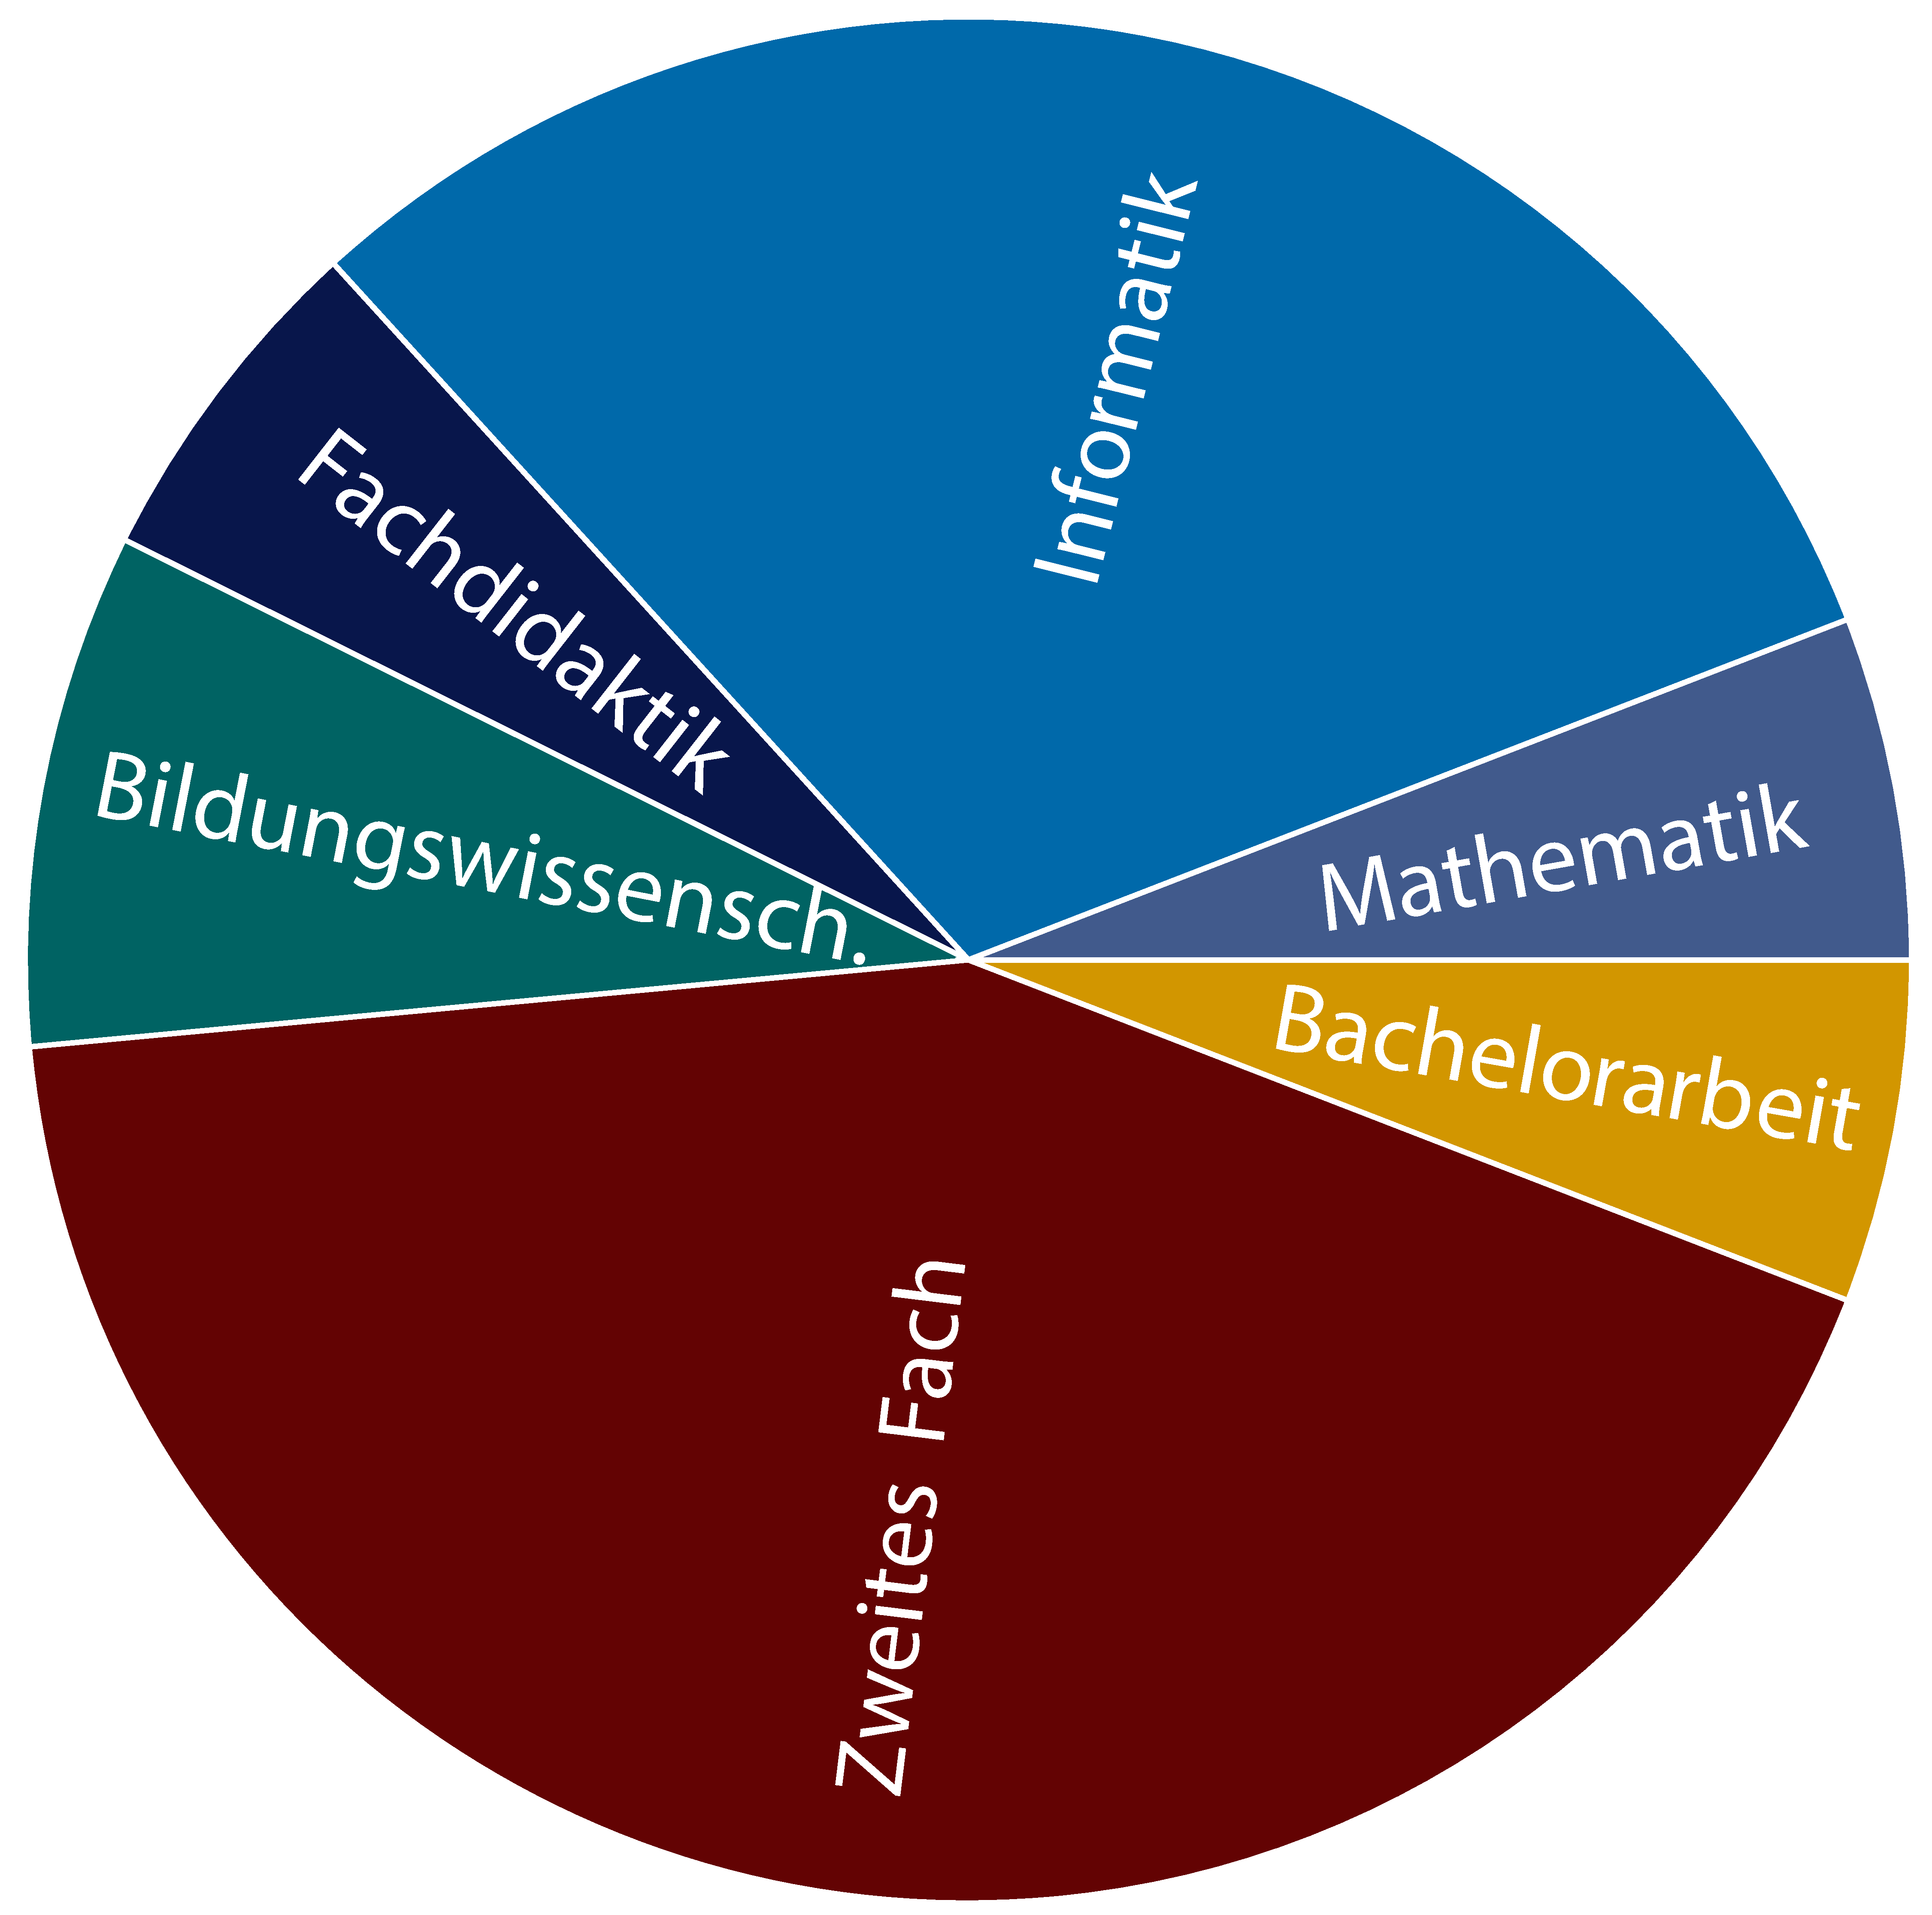
\includegraphics[width=0.4\textwidth]{images/lehramt_informatik_piechartonly.pdf}
			\caption{Verteilung der Themenbereiche über das komplette Studium}
		\end{figure}
	\end{block}
	
	\begin{block}{Was macht man in welchem Semester?}
		\begin{figure}[h!]
			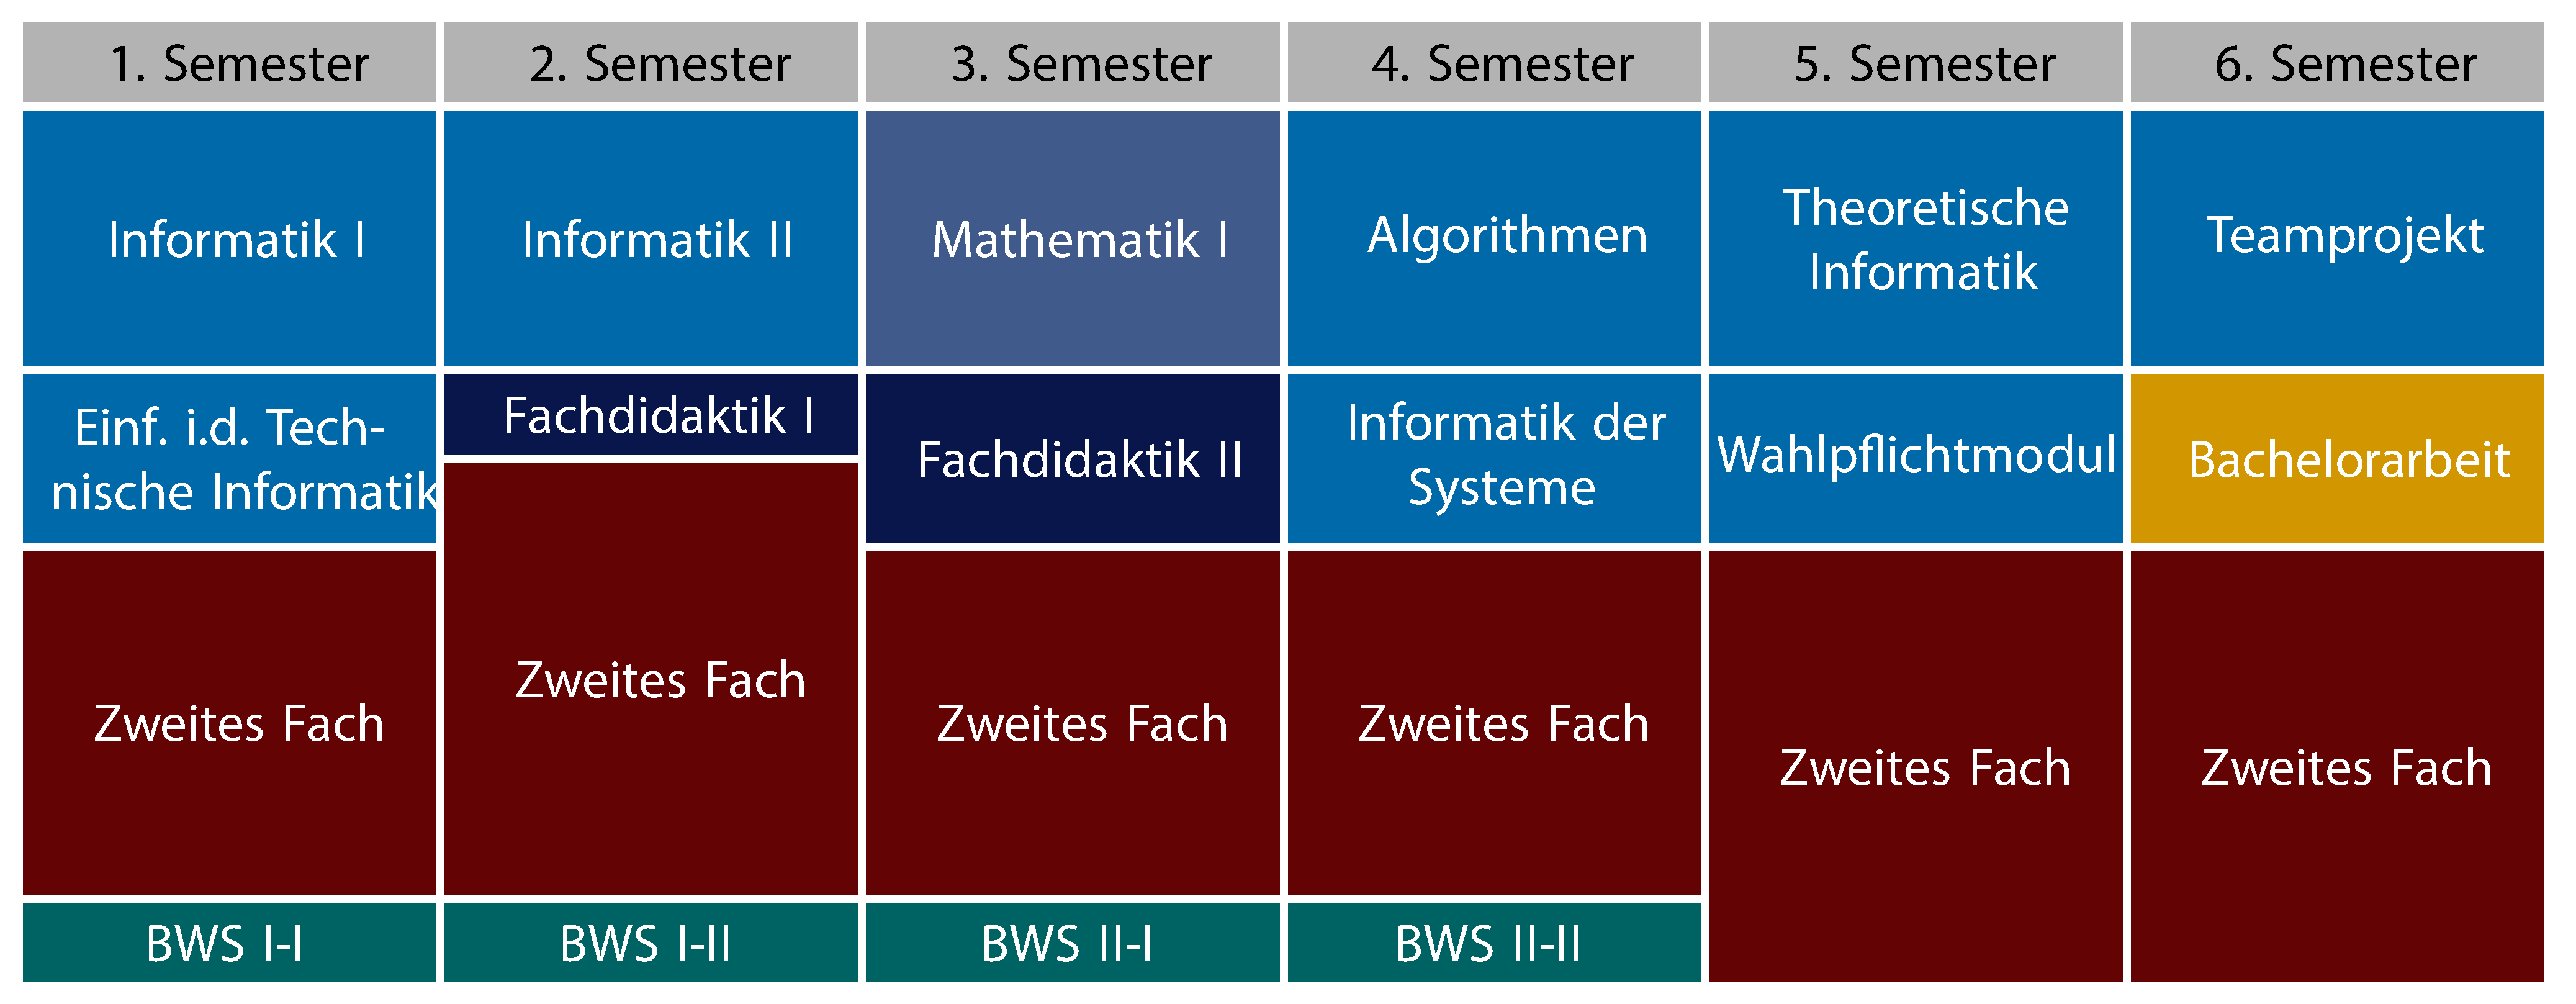
\includegraphics[width=\textwidth]{images/lehramt_informatik_Studienplanonly.pdf}
		\end{figure}
		Das 1. Semester ist nach Plan ein Wintersemester. Wenn du dein Studium zum Sommersemester beginnen möchtest, beginnst du im Plan bei Semester 2 und machst dann Semester 1. 
		Dieser Verlauf ist unabhängig vom Studienbeginn nur ein Vorschlag und kein bindender Studienplan. Es empfiehlt sich jedoch, den Plan einzuhalten, wenn man in Regelstudienzeit studieren möchte.
	\end{block}
\vfill
\begin{flushright}
	
\includegraphics[width=0.4\textwidth]{images/fsilogo.pdf}
\end{flushright}
